\chapter{Generating random performance tableaux}
\label{sec:5}

\abstract*{To be written.}

\abstract{To be written.}

\section{Introduction}
\label{sec:5.1}

The {\tt randomPerfTabs} module provides several constructors for generating random performance tableaux models of different kind, mainly for the purpose of testing implemented methods and tools presented and discussed in the Algorithmic Decision Theory course at the University of Luxembourg. This tutorial concerns the most useful models.

The simplest model, called \textbf{RandomPerformanceTableau}, generates a set of $n$ decision actions, a set of $m$ real-valued performance criteria, ranging by default from $0.0$ to $100.0$, associated with default discrimination thresholds: $2.5$ (ind.), $5.0$ (pref.) and $60.0$ (veto). The generated performances are Beta(2,2) distributed on each measurement scale.

One of the most useful models, called \textbf{RandomCBPerformanceTableau}, proposes a performance tableau involving two decision objectives, named \emph{Costs} (to be minimized) respectively \emph{Benefits} (to be maximized); its purpose being to generate more or less contradictory performances on these two, usually conflicting, objectives. \emph{Low costs} will randomly be coupled with \emph{low benefits}, whereas \emph{high costs} will randomly be coupled with \emph{high benefits}.

Many public policy decision problems involve three often conflicting decision objectives taking into account \emph{economical}, \emph{societal} as well as \emph{environmental} aspects. For this type of performance tableau model, we provide a specific model, called \textbf{Random3ObjectivesPerformanceTableau}.

Deciding which students, based on the grades obtained in a number of examinations, validate or not their academic studies, is the genuine decision practice of universities and academies. To thouroughly study these kind of decision problems, we provide a corresponding performance tableau model, called \textbf{RandomAcademicPerformanceTableau}, which gathers grades obtained by a given number of students in a given number of weighted courses.    

In order to study aggregation of election results (see Chapter \ref{sec:7}) in the context of bipolar-valued outranking digraphs, we provide furthermore a specific performance tableau model called \textbf{RandomRankPerformanceTableau} which provides ranks (linearly ordered performances without ties) of a given number of election candidates (decision actions) for a given number of weighted voters (performance criteria).
 
\section{Random standard performance tableaux}
\label{sec:5.2}
    
The {\tt RandomPerformanceTableau} class, the simplest of the kind, specializes the generic {\tt PerformanceTableau} class, and takes the following parameters:
\begin{itemize}
\item \texttt{numberOfActions} := nbr of decision actions.
\item \texttt{numberOfCriteria} := number performance criteria.
\item \texttt{weightDistribution} := 'random' (default) | 'fixed' | 'equisignificant':
      \begin{itemize}
         \item If 'random', weights are uniformly selected randomly from the given weight scale;
         \item If 'fixed', the weightScale must provided a corresponding weights distribution;
         \item If 'equisignificant', all criterion weights are put to unity.
      \end{itemize}
\item \texttt{weightScale} := [Min,Max] (default =(1,numberOfCriteria).
\item \texttt{IntegerWeights} := True (default) | False (normalized to proportions of 1.0).
\item \texttt{commonScale} := [a,b]; common performance measuring scales (default = [0.0,100.0])
\item \texttt{commonThresholds} := $[(q0,q1),(p0,p1),(v0,v1)]$; common indifference($q$), preference ($p$) and considerable performance difference ($v$) discrimination thresholds. For each threshold type $x \in \{q,p,v\}$, the float $x0$ value represents a constant percentage of the common scale and the float $x1$ value a proportional value of the actual performance measure. Default values are $[(2.5.0,0.0),(5.0,0.0),(60.0,0,0)]$. 
\item \texttt{commonMode} := common random distribution of random performance measurements (default = ('beta',None,(2,2)) ):
      \begin{itemize}
         \item  ('uniform', None, None), uniformly distributed float values on the given common scales' range [Min,Max];
         \item ('normal', $\mu$, $\sigma$), truncated Gaussian distribution, by default $\mu = (b-a)/2$ and $\sigma = (b-a)/4$;
         \item ('triangular', \emph{mode}, \emph{repartition}), generalized triangular distribution with a probability repartition parameter specifying the probability mass accumulated until the mode value. By default, \emph{mode} = $(b-a)/2$ and *repartition* = 0.5.
         \item ('beta',None,(alpha,beta)), a beta generator with default alpha=2 and beta=2 parameters.
      \end{itemize}
\item \texttt{valueDigits} := integer, precision of performance measurements (2 decimal digits by default).
\item \texttt{missingDataProbability} := $0.0 \leq \mathtt{float} \leq 1.0$ ; probability of missing performance evaluation on a criterion for an alternative (default $0.025$).
\item \texttt{NA} := \texttt{Decimal} (default = $-999$); missing data symbol. 
\end{itemize} 

\noindent \textbf{Code example:}

\begin{lstlisting}[caption={Generating a random performance tableau},label=list:5.1,basicstyle=\footnotesize]
>>> from randomPerfTabs import RandomPerformanceTableau
>>> t = RandomPerformanceTableau(numberOfActions=21,\
...                 numberOfCriteria=13,seed=100)
>>> t.actions
 {'a01': {'comment': 'RandomPerformanceTableau() generated.',
	'name': 'random decision action'},
	 'a02': { ... },
    ...
   }
>>> t.criteria
{'g01': {'thresholds': {
      'ind' : (Decimal('10.0'), Decimal('0.0')),
      'veto': (Decimal('80.0'), Decimal('0.0')),
      'pref': (Decimal('20.0'), Decimal('0.0'))},
      'scale': [0.0, 100.0],
      'weight': Decimal('1'),
     'name': 'digraphs.RandomPerformanceTableau() instance',
     'comment': 'Arguments: ; weightDistribution=random;
         weightScale=(1, 1); commonMode=None'},
	 'g02':  { ... },
     ... }
>>> t.evaluation
 {'g01': {'a01': Decimal('15.17'),
      'a02': Decimal('44.51'),
      'a03': Decimal('-999'),  # missing evaluation
       ...  },
   ...
 }
>>> t.showHTMLPerformanceTableau()
 \end{lstlisting}

\begin{figure}[h]
%\sidecaption
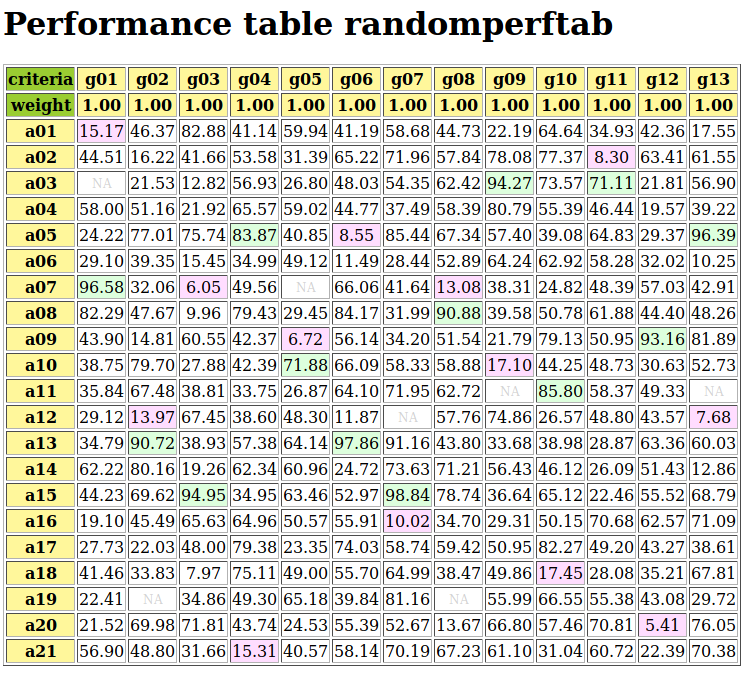
\includegraphics[width=10cm]{Figures/randomPerfTab1.png}
\caption{Browser view on random performance tableau instance}
\label{fig:5.1}       % Give a unique label
\end{figure}

Notice that missing (\texttt{NA}) evaluation are registered in a performance tableau by default as \texttt{Decimal('-999')} value (see Listing \ref{list:5.1} Line 24). Best and worst performance on each criterion are marked in \emph{light green}, respectively in \emph{light red}.
	    
\section{Random Cost-Benefit performance tableaux}
\label{sec:5.3}

We provide the \texttt{RandomCBPerformanceTableau} class for generating random \emph{Costs} versus \emph{Benefits} organized performance tableaux following the directives below:
\begin{itemize}
\item We distinguish three types of decision actions: \emph{cheap}, \emph{neutral} and \emph{expensive} ones with an equal proportion of 1/3. We also distinguish two types of weighted criteria: \emph{Costs} criteria to be \emph{minimized}, and \emph{Benefits} criteria to be \emph{maximized}; in the proportions 1/3 respectively 2/3. 
\item  Random performances on each type of criteria  are drawn, either from an ordinal scale $[0;10]$, or from a cardinal scale $[0.0;100.0]$, following a parametric triangular law of mode: $30\%$ performance for cheap, $50\%$ for neutral, and $70\%$ performance for expensive decision actions, with constant probability repartition $0.5$ on each side of the respective mode. 
\item Costs criteria use mostly cardinal scales (3/4), whereas Benefits criteria use mostly ordinal scales (2/3). 
\item  The sum of weights of the Costs criteria by default equals the sum weights of the Benefits criteria: \texttt{weighDistribution} = 'equiobjectives'. 
\item On cardinal criteria, both of cost or of benefit type, we observe following constant preference discrimination quantiles: $5\%$ indifferent situations, $90\%$ strict preference situations, and $5\%$ veto situation. 
\end{itemize}

\textbf{Parameters}:
\begin{itemize}
\item If \texttt{numberOfActions == None}, a uniform random number between 10 and 31 of cheap, neutral or advantageous actions (equal 1/3 probability each type) actions is instantiated;
\item If \texttt{numberOfCriteria == None}, a uniform random number between 5 and 21 of cost or benefit criteria (1/3 respectively 2/3 probability) is instantiated;
\item \emph{weightDistribution} := {'equiobjectives'|'fixed'|'random'|'equisignificant' (default = 'equisignificant')};
\item default \texttt{weightScale} for 'random' weight distribution is 1 - \texttt{numberOfCriteria};
\item All cardinal criteria are evaluated with decimals between $0.0$ and $100.0$ whereas ordinal criteria are evaluated with integers between 0 and 10.
\item \texttt{commonThresholds} is obsolete. Preference discrimination is specified as percentiles of concerned performance differences (see below).
\item \texttt{commonPercentiles} := {'ind':5, 'pref':10, 'veto':95} are expressed in percents (reversed for vetoes) and only concern cardinal criteria.
\item \texttt{missingDataProbability} := $0.0 \leq \mathtt{float} \leq 1.0$ ; probability of missing performance evaluation on a criterion for an alternative (default $0.025$).
\item \texttt{NA} := \texttt{Decimal} (default = $-999$); missing data symbol. 
\end{itemize}

Minimal number of decision actions required is 3 ! 

\noindent \textbf{Example Python session}:

\begin{lstlisting}[caption={Generating a random Cost-Benefit performance tableau},label=list:5.2]
>>> from randomPerfTabs import RandomCBPerformanceTableau
>>> t = RandomCBPerformanceTableau(
 ...       numberOfActions=7,\
   ...       numberOfCriteria=5,\
   ...       weightDistribution='equiobjectives',\
   ...       commonPercentiles={'ind':0.05,'pref':0.10,'veto':0.95},\
   ...       seed=100)

>>> t.showActions()
 *----- show decision action --------------*
    key:  a1
      short name: a1
      name:       random cheap decision action
    key:  a2
      short name: a2
      name:       random neutral decision action
    ...
    key:  a7
      short name: a7
      name:       random advantageous decision action
>>> t.showCriteria()
    *----  criteria -----*
    g1 'random ordinal benefit criterion'
      Scale = (0, 10)
      Weight = 2
    ...
    g2 'random cardinal cost criterion'
      Scale = (0.0, 100.0)
      Weight = 3 
      Threshold ind  :  1.76 + 0.00x ; percentile:   9.5
      Threshold pref :  2.16 + 0.00x ; percentile:  14.3
      Threshold veto : 73.19 + 0.00x ; percentile:  95.2
    ...
 \end{lstlisting}

In the example above, we may notice the three types of decision actions (see Listing \ref{list:5.2} Lines 10-20), as well as the two types (Lines 22-32) of criteria with either an \emph{ordinal} or a \emph{cardinal} performance measuring scale. In the latter case, by default about $5\%$ of the random performance differences will be below the \emph{indifference} and $10\%$ below the \emph{preference} discriminating threshold. About $5\%$ will be considered as \emph{considerably large}. More statistics about the generated performances is available as follows.
\begin{lstlisting}
>>> t.showStatistics()
    *-------- Performance tableau summary statistics -------*
    Instance name      : randomCBperftab
    Actions            : 7
    Criteria           : 5
     Criterion name       : g1
       Criterion weight     : 2
       criterion scale    : 0.00 - 10.00
       mean evaluation    : 5.14
       standard deviation : 2.64
       maximal evaluation : 8.00
       quantile Q3 (x_75) : 8.00
       median evaluation  : 6.50
       quantile Q1 (x_25) : 3.50
       minimal evaluation : 1.00
       mean absolute difference      : 2.94
       standard difference deviation : 3.74
     Criterion name       : g2
       Criterion weight     : 3
       criterion scale    : -100.00 - 0.00
       mean evaluation    : -49.32
       standard deviation : 27.59
       maximal evaluation : 0.00
       quantile Q3 (x_75) : -27.51
       median evaluation  : -35.98
       quantile Q1 (x_25) : -54.02
       minimal evaluation : -91.87
       mean absolute difference      : 28.72
       standard difference deviation : 39.02
     ...
\end{lstlisting}

A (potentially ranked) colored heatmap with 5 color levels is also provided.
\begin{lstlisting}[basicstyle=\footnotesize]
   >>> t.showHTMLPerformanceHeatmap(colorLevels=5,rankingRule=None)
 \end{lstlisting}

 \begin{figure}[h]
%\sidecaption
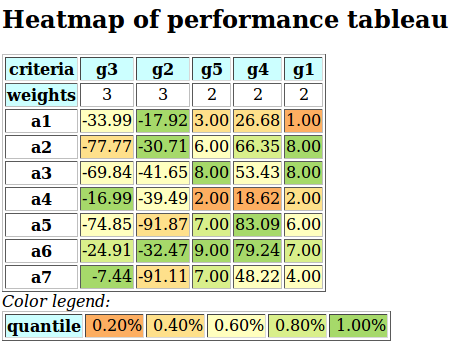
\includegraphics[width=8cm]{Figures/randomCBHeatmap.png}
\caption{Unranked heatmap of a random Cost-Benefit performance tableau}
\label{fig:5.2}       % Give a unique label
\end{figure}
 
Such a performance tableau may be stored and re-accessed as follows.

\begin{lstlisting}[basicstyle=\footnotesize]
>>> t.save('temp')
    *----- saving performance tableau in XMCDA 2.0 format  -------------*
    File: temp.py saved !
>>> from perfTabs import PerformanceTableau
>>> t = PerformanceTableau('temp')
\end{lstlisting}

 If needed for instance in an R session, a CSV version of the performance tableau may be created as follows.
\begin{lstlisting}
>>> t.saveCSV('temp')
    * --- Storing performance tableau in CSV format in file temp.csv
\end{lstlisting}

We may inspect the content of the file \emph{temp.csv} in a shell console:
\begin{lstlisting}
...\% less temp.csv
    "actions","g1","g2","g3","g4","g5"
    "a1",1.00,-17.92,-33.99,26.68,3.00
    "a2",8.00,-30.71,-77.77,66.35,6.00
    "a3",8.00,-41.65,-69.84,53.43,8.00
    "a4",2.00,-39.49,-16.99,18.62,2.00
    "a5",6.00,-91.87,-74.85,83.09,7.00
    "a6",7.00,-32.47,-24.91,79.24,9.00
    "a7",4.00,-91.11,-7.44,48.22,7.00
\end{lstlisting}

 \section{Random three objectives performance tableaux}
\label{sec:5.4}

We provide the \texttt{Random3ObjectivesPerformanceTableau} class for generating random performance tableaux concerning potential public policies evaluated with respect to three preferential decision objectives taking respectively into account \emph{economical}, \emph{societal} as well as \emph{environmental} aspects.

Each public policy is qualified randomly as performing \emph{weak} ($-$), \emph{fair} ($\sim$) or \emph{good} ($+$) on each of the three objectives. 

Generator directives are the following:
\begin{itemize}
\item \texttt{numberOfActions} = $20$ (default),
\item \texttt{numberOfCriteria} = $13$ (default),
\item \texttt{weightDistribution} = 'equiobjectives' (default) | 'random' | 'equisignificant',
\item \texttt{weightScale} = (1,\texttt{numberOfCriteria}): only used when random criterion weights are requested,
\item \texttt{integerWeights} = True (default): False gives normalized rational weights, 
\item \texttt{commonScale} = ($0.0$,$100.0$),
\item \texttt{commonThresholds} = [$(5.0,0.0)$,$(10.0,0.0)$,$(60.0,0.0)$]: Performance discrimination thresholds may be set for 'ind', 'pref' and 'veto' thresholds,  
\item \texttt{commonMode} = ['triangular','variable',$0.5$]: random number generators of various other types ('\emph{uniform}','\emph{beta}') are available. If the mode of the 'triangular' distribution is set to 'variable', three modes at $0.3 (-)$, $0.5 (\sim)$, respectively $0.7 (+)$ of the common scale span are set at random for each coalition and action. 
\item \texttt{valueDigits} = 2 (default): evaluations are encoded as decimals,
\item \texttt{missingDataProbability} = $0.05$ (default): random insertion of missing values with given probability,  
\item \texttt{NA} := \texttt{Decimal} (default = $-999$); missing data symbol,
\item \texttt{seed} = None (default). 
\end{itemize}
Minimal number of decision actions required is 3! 

\noindent \textbf{Example Python session:}
\begin{lstlisting}[caption={Generating a random 3 Objectives performance tableau},label=list:5.3]
>>> from randomPerfTabs import Random3ObjectivesPerformanceTableau
>>> t = Random3ObjectivesPerformanceTableau(\
...              numberOfActions=31,\
...              numberOfCriteria=13,\
...              weightDistribution='equiobjectives',\
...              seed=120)
>>> t.showObjectives()
  *------ show objectives -------*
    'Eco': Economical aspect
     'ec04' criterion of objective 'Eco' 20
     'ec05' criterion of objective 'Eco' 20
     'ec08' criterion of objective 'Eco' 20
     'ec11' criterion of objective 'Eco' 20
      Total weight: 80.00 (4 criteria)
    'Soc': Societal aspect
     'so06' criterion of objective 'Soc' 16
     'so07' criterion of objective 'Soc' 16
     'so09' criterion of objective 'Soc' 16
     's010' criterion of objective 'Soc' 16
     's013' criterion of objective 'Soc' 16
      Total weight: 80.00 (5 criteria)
    'Env': Environmental aspect
     'en01' criterion of objective 'Env' 20
     'en02' criterion of objective 'Env' 20
     'en03' criterion of objective 'Env' 20
     'en12' criterion of objective 'Env' 20
    Total weight: 80.00 (4 criteria)
\end{lstlisting}
In Listing \ref{list:5.3} above, we notice that 5 \emph{equisignificant} criteria ('so06', 'so07', 'so09', 'so10', 'so13') evaluate for instance the performance of the public policies from a \emph{societal} point of view (Lines 15-21). 4 \emph{equisignificant} criteria do the same from an \emph{economical} (Lines 9-14), respectively an \emph{environmental} point of view (Lines 22-27). The '\texttt{equiobjectives}' directive results hence in a balanced total weight (80.00) for each decision objective. 
\begin{lstlisting}
>>> t.showActions()
  key:  'p01'
    name:       random public policy Eco+ Soc- Env+
    profile:    {'Eco': 'good', 'Soc': 'weak', 'Env': 'good'}
  key:  'p02'
    ...
  key:  'p26'
    name:       random public policy Eco+ Soc+ Env-
    profile:    {'Eco': 'good', 'Soc': 'good', 'Env': 'weak'}
    ...
  key:  'p30'
    name:       random public policy Eco- Soc- Env-
    profile:    {'Eco': 'weak', 'Soc': 'weak', 'Env': 'weak'}
    ...
 \end{lstlisting}
  
Variable triangular modes ($0.3$, $0.5$ or $0.7$ of the span of the measure scale) for each objective result in different performance status for each public policy with respect to the three objectives. Policy 'p01', for instance, will probably show \emph{good} performances wrt the \emph{economical}  and environmental aspects, and \emph{weak} performances wrt the \emph{societal} aspect.

For testing purposes we provide a special \texttt{PartialPerformanceTableau} class for extracting a partial performance tableau from a given tableau instance. In the example blow, we may construct the partial performance tableaux corresponding to each one of the three decision objectives.
\begin{lstlisting}
>>> from perfTabs import PartialPerformanceTableau
>>> teco = PartialPerformanceTableau(t,criteriaSubset=\
...                           t.objectives['Eco']['criteria'])
>>> tsoc = PartialPerformanceTableau(t,criteriaSubset=\
...                           t.objectives['Soc']['criteria'])
>>> tenv = PartialPerformanceTableau(t,criteriaSubset=\
...                           t.objectives['Env']['criteria'])
\end{lstlisting}

One may thus compute a partial bipolar-valued outranking digraph for each individual objective.
\begin{lstlisting}
>>> from outrankingDigraphs import BipolarOutrankingDigraph
>>> geco = BipolarOutrankingDigraph(teco)
>>> gsoc = BipolarOutrankingDigraph(tsoc)
>>> genv = BipolarOutrankingDigraph(tenv)
\end{lstlisting}

The three partial digraphs: $geco$, $gsoc$ and $genv$,  hence model the preferences represented in each one of the partial performance tableaux. And, we may aggregate these three outranking digraphs with an epistemic fusion operator.
\begin{lstlisting}[basicstyle=\scriptsize]
>>> from digraphs import FusionLDigraph
>>> gfus = FusionLDigraph([geco,gsoc,genv])
>>> gfus.strongComponents()
  {frozenset({'p30'}), 
   frozenset({'p10','p03','p19','p08','p07','p04',
    'p21','p20','p13','p23','p16','p12','p24','p02',
    'p31','p29','p05','p09','p28','p25','p17','p14',
    'p15','p06','p01','p27','p11','p18','p22'}), 
   frozenset({'p26'})
  }
>>> from digraphs import StrongComponentsCollapsedDigraph
>>> scc = StrongComponentsCollapsedDigraph(gfus)
>>> scc.showActions()
  *----- show digraphs actions --------------*
  key:  frozenset({'p30'})
    short name: Scc_1
    name:  _p30_
    comment:    collapsed strong component
  key:  frozenset({'p10','p03','p19','p08','p07','p04','p21','p20','p13',
                   'p23','p16','p12','p24','p02','p31','p29','p05','p09','p28','p25',
                   'p17','p14','p15','p06','p01','p27','p11','p18','p22'})
    short name: Scc_2
    name: _p10_p03_p19_p08_p07_p04_p21_p20_p13_p23_p16_p12_p24_p02_p31_\
           p29_p05_p09_p28_p25_p17_p14_p15_p06_p01_p27_p11_p18_p22_
    comment:    collapsed strong component
  key:  frozenset({'p26'})
    short name: Scc_3
    name:  _p26_
    comment:    collapsed strong component
\end{lstlisting}

A graphviz drawing illustrates the apparent preferential links between the strong components.
\begin{lstlisting}[basicstyle=\footnotesize]
   >>> scc.exportGraphViz('scFusionObjectives')
    *---- exporting a dot file for GraphViz tools ----*
    Exporting to scFusionObjectives.dot
    dot -Grankdir=BT -Tpng scFusionObjectives.dot\
                     -o scFusionObjectives.png
\end{lstlisting}
\begin{figure}[h]
\sidecaption
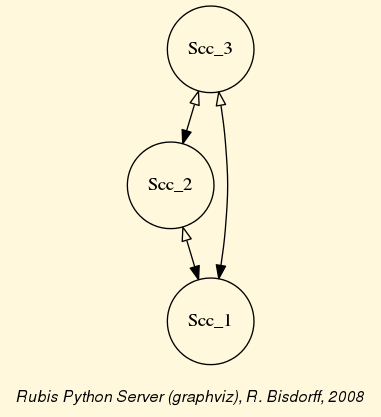
\includegraphics[width=6cm]{Figures/sccFusionObjectives.png}
\caption{Strong components digraph. Public policy 'p26' (Eco+ Soc+ Env-) appears dominating the other policies, whereas policy 'p30' (Eco- Soc- Env-) appears to be dominated by all the others.}
\label{fig:5.3}       % Give a unique label
\end{figure}
	   

\section{Random academic performance tableaux}
\label{sec:5.5}

The \texttt{RandomAcademicPerformanceTableau} class generates temporary performance tableaux with random grades for a given number of students in different courses. 

\noindent Generator directives:
\begin{itemize}
\item \texttt{numberOfStudents} := \texttt{Integer} (default 10)
\item \texttt{numberOfCourses} := \texttt{Integer} (default 5)
\item \texttt{weightDistribution} := '\emph{equisignificant}' | '\emph{random}' (default),
\item \texttt{weightScale} := $1$, $1$ - \texttt{numberOfCourses} (default when random)),
\item \texttt{IntegerWeights} := \texttt{Boolean} (True = default),
\item \texttt{commonScale} := (\texttt{Integer},\texttt{integer}) $(0,20)$ (default),
\item \texttt{ndigits} := \texttt{Integer} (default 0),
\item \texttt{WithTypes} := \texttt{Boolean} (default False),
\item \texttt{commonMode} := ('\emph{triangular}',$xm$=14,$r$=0.25) (default),
\item \texttt{commonThresholds} := {'ind':(0,0), 'pref':(1,0)} (default),
\item \texttt{missingDataProbability} := 0.0 (default),
\item \texttt{NA} := \texttt{Decimal} (default = $-999$); missing data symbol. 
\end{itemize}      

When parameter \texttt{WithTypes} is set to \emph{True}, the students are randomly allocated to one of the four categories: \emph{weak} (1/6), \emph{fair} (1/3), \emph{good} (1/3), and \emph{excellent} (1/3), in the bracketed proportions. In a default $0-20$ grading range, the random range of a weak student is $0-10$, of a fair student $4-16$, of a good student $8-20$, and of an excellent student $12-20$. The random grading generator follows in this case a double triangular probablity law with \emph{mode} ($xm$) equal to the middle of the random range and median repartition ($r = 0.5$) of probability each side of the mode.

\begin{lstlisting}[caption={Generating a random academic performance tableau},label=list:5.5]
>>> from randomPerfTabs import RandomAcademicPerformanceTableau
>>> t = RandomAcademicPerformanceTableau(\
...        numberOfStudents=11,\
...        numberOfCourses=7, missingDataProbability=0.03,\
...        WithTypes=True, seed=100)
>>> t
  *------- PerformanceTableau instance description ------*
   Instance class   : RandomAcademicPerformanceTableau
   Seed             : 100
   Instance name    : randstudPerf
   Actions          : 11
   Criteria         : 7
   Attributes       : ['randomSeed', 'name', 'actions',
             'criteria', 'evaluation', 'weightPreorder']
>>> t.showPerformanceTableau()
  *----  performance tableau -----*
   Courses |   'm1'  'm2'  'm3'  'm4'  'm5'  'm6'  'm7' 
     ECTS  |    2     1     3     4     1     1     5    
  ---------|------------------------------------------
    's01f' |    12    13    15    08    16    06    15   
    's02g' |    10    15    20    11    14    15    18   
    's03g' |    14    12    19    11    15    13    11   
    's04f' |    13    15    12    13    13    10    06   
    's05e' |    12    14    13    16    15    12    16   
    's06g' |    17    13    10    14    NA    15    13   
    's07e' |    12    12    12    18    NA    13    17   
    's08f' |    14    12    09    13    13    15    12   
    's09g' |    19    14    15    13    09    13    16   
    's10g' |    10    12    14    17    12    16    09   
    's11w' |    10    10    NA    10    10    NA    08
>>> t.weightPreorder
  [['m2', 'm5', 'm6'], ['m1'], ['m3'], ['m4'], ['m7']]
\end{lstlisting}
  
The example tableau, generated for instance above with \texttt{missingDataProbability} = $0.03$, *\texttt{WithTypes} = True and \texttt{seed} = 100 (see Listing \ref{list:5.5} Lines 2-5), results in a set of two excellent ('s05e', 's07e'), five good ('s02g', 's03g', s06g, 's09g', 's10g'), three fair ('s01f', 's04f', 's08f') and one weak ('s11w') student performances. Notice that six students get a grade below the course validating threshold 10 and we observe four missing grades (\texttt{NA}), two in course 'm5' and, one in courses 'm3' and 'm6' (see Lines 20-30).

We may show a statistical summary of the students' grades obtained in the heighest weighted course, namely 'm7', followed by a performance heatmap browser view showing a global ranking of the students' performances from best to weakest.
\begin{lstlisting}[caption={Student performance summary statistics per course},label=list:5.6]
>>> t.showCourseStatistics('m7')
  *----- Summary performance statistics ------*
   Course name    : g7
   Course weight  : 5
   Students       : 11
   Grading scale  : 0.00 - 20.00
   Missing evaluations : 0
   Mean evaluation       : 12.82
   Standard deviation    : 3.79
   Maximal evaluation    : 18.00
   Quantile Q3 (x_75)    : 16.25
   Median evaluation     : 14.00
   Quantile Q1 (x_25)    : 10.50
   Minimal evaluation    : 6.00
   Mean absolute difference      : 4.30
   Standard difference deviation : 5.35
>>> t.showHTMLPerformanceHeatmap(colorLevels=5,\
...                  pageTitle='Ranking the students')
\end{lstlisting}
\begin{figure}[h]
\sidecaption
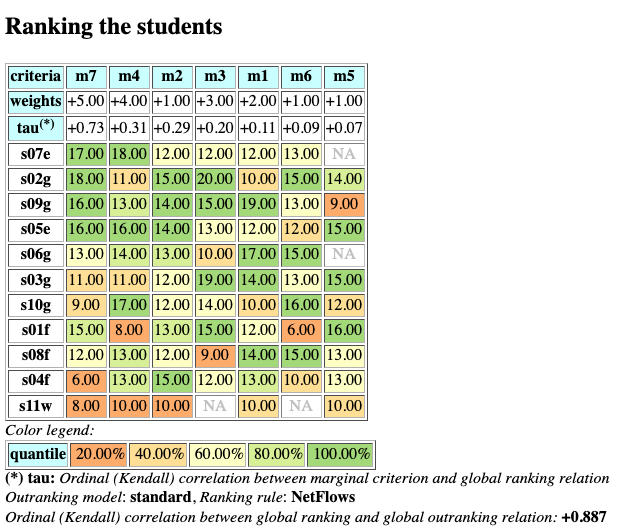
\includegraphics[width=6cm]{Figures/rankingStudents.png}
\caption{Ranking the students with a performance heatmap view. The ranking shown here is produced with the default \emph{NetFlows} ranking rule}
\label{fig:5.4}       % Give a unique label
\end{figure}

With a mean marginal correlation of $+0.361$ (see Listing \ref{list:5.5} Lines 17-) associated with a low standard deviation ($0.248$), the result represents a rather \emph{fair weighted consensus} made between the individual courses' marginal rankings.
\begin{lstlisting}[caption={Consensus quality of the students's ranking},label=list:5.7]
>>> from outrankingDigraphs import\
...                  BipolarOutrankingDigraph
>>> g = BipolarOutrankingDigraph(t)
>>> t.showRankingConsensusQuality(\
...                 g.computeNetFlowsRanking())
  Consensus quality of ranking:
  ['s07', 's02', 's09', 's05', 's06', 's03', 's10',
   's01', 's08', 's04', 's11']
  Criterion (weight): correlation
  -------------------------------
     'm7' (0.294): +0.727
     'm4' (0.235): +0.309
     'm2' (0.059): +0.291
     'm3' (0.176): +0.200
     'm1' (0.118): +0.109
     'm6' (0.059): +0.091
     'm5' (0.059): +0.073
  Summary:
   Weighted mean marginal correlation (a): +0.361
   Standard deviation (b)                : +0.248
   Ranking fairness (a)-(b)              : +0.113
\end{lstlisting}
   
\section{Random linearly ranked performance tableaux}
\label{sec:5.6}

Finally, we provide the \texttt{RandomRankPerformanceTableau} class for generating multiple criteria ranked performance tableaux, i.e. on each criterion, all decision action's evaluations appear linearly ordered without ties.

This type of random performance tableau is matching the \texttt{RandomLinearVotingProfile} class provided by the \texttt{votingProfiles} module.  
        
Parameters:
\begin{itemize}
\item \texttt{numberOfActions},
\item \texttt{numberOfCriteria},
\item \texttt{weightDistribution} := 'equisignificant' | 'random' (default),
\item \texttt{weightScale} := (1, 1 | numberOfCriteria (default when random)),
\item \texttt{integerWeights} := Boolean (True = default),
\item \texttt{commonThresholds} := \{'ind':(0,0), 'pref':(1,0), 'veto':(numberOfActions,0)\}. (default) 
\end{itemize}


Concluding remarks an transition to Chapter 6. 